\documentclass[10pt]{beamer}

%% Based on the original theme by Matthias Vogelgesang

\usetheme[progressbar=frametitle]{metropolis}
\usepackage{appendixnumberbeamer}

\usepackage{booktabs}
\usepackage[scale=2]{ccicons}

\usepackage{pgfplots}
\usepgfplotslibrary{dateplot}

\usepackage{xspace}
\newcommand{\themename}{\textbf{\textsc{metropolis}}\xspace}

%%%%%%%%%%%%%%%%%%%%%%%%%%%%
%% UNCC Theme Adjustments %%
%%%%%%%%%%%%%%%%%%%%%%%%%%%%
\definecolor{CanvasBG}{HTML}{FAFAFA}

% From the official style guide
\definecolor{UnccGreen}{HTML}{00703C}
\definecolor{UnccGold}{HTML}{B3A369}
\definecolor{UnccLightGreen}{HTML}{C3D7A4}
\definecolor{UnccYellow}{HTML}{F0CB00}
\definecolor{UnccOrange}{HTML}{F3901D}
\definecolor{UnccLightYellow}{HTML}{FFF6DC}
\definecolor{UnccBlue}{HTML}{00728F}
\definecolor{UnccPink}{HTML}{DE3A6E}
\definecolor{White}{HTML}{FFFFFF}
\definecolor{LightGray}{HTML}{DDDDDD}

% Supporting Color Palette
\definecolor{WarmGray}{HTML}{696158}
\definecolor{StoneGray}{HTML}{717C7D}
\definecolor{DarkGreen}{HTML}{2C5234}
\definecolor{LightGreen}{HTML}{509E2F}
\definecolor{BrightGold}{HTML}{F0CB00}

% Screamers
\definecolor{Royal}{HTML}{72246C}
\definecolor{Ocean}{HTML}{006BA6}
\definecolor{Flash}{HTML}{B52555}
\definecolor{Citrus}{HTML}{FFB81C}
\definecolor{Spring}{HTML}{CEDC00}

% Serenity
\definecolor{Garden}{HTML}{B7CE95}
\definecolor{Sand}{HTML}{F0E991}
\definecolor{Bloom}{HTML}{F1E6B2}
\definecolor{Clay}{HTML}{B7B09C}
\definecolor{Cloud}{HTML}{BAC5B9}

% Set colors here
\setbeamercolor{frametitle}{bg=UnccGreen}
\setbeamercolor{progress bar}{bg=BrightGold, fg=UnccGreen}
\setbeamercolor{alerted text}{fg=Flash}

\setbeamercolor{block title}{bg=LightGreen, fg=White}
\setbeamercolor{block title example}{bg=Ocean, fg=White}
\setbeamercolor{block title alerted}{bg=Citrus, fg=White}
\setbeamercolor{block body}{bg=CanvasBG}

\metroset{titleformat=smallcaps, progressbar=foot, sectionpage=none}

\makeatletter
\setlength{\metropolis@progressinheadfoot@linewidth}{2pt}
\setlength{\metropolis@titleseparator@linewidth}{2pt}
\setlength{\metropolis@progressonsectionpage@linewidth}{2pt}
%%%%%%%%%%%%%%%%%%%%%%%%%%%%
%% UNCC Theme Adjustments %%
%%%%%%%%%%%%%%%%%%%%%%%%%%%%


\title{Abschlussvortrag}
\subtitle{Handgestenerkennung mit Entscheidungsbäumen}
% \date{\today}
\date{17.03.2021}
\author{Tom Dymel}
\institute{Forschungsprojekt und Seminar\\Technische Universität Hamburg}
% \titlegraphic{\hfill\includegraphics[height=1.5cm]{logo.pdf}}

\begin{document}

\maketitle

\section{Motivation}
\begin{frame}{Motivation}
\begin{itemize}
    \item Zuverlässige Gestenerkennung auf Mikrocontroller
    \item Preiswertes Modul
    \item Echtzeit-Evaluierung 
    \item Vorherige Ansätze:
    \begin{itemize}
        \item FFNN (Engelhardt, Kubik, Giese)
        \item RNN (Klisch, Engelhardt)
    \end{itemize}
    \item Entscheidungsbäume potentiell effizienter
\end{itemize}
\end{frame}

\section{Optische Handgestenerkennung}
%Kurz!
\begin{frame}{Optische Handgestenerkennung}
\begin{figure}
    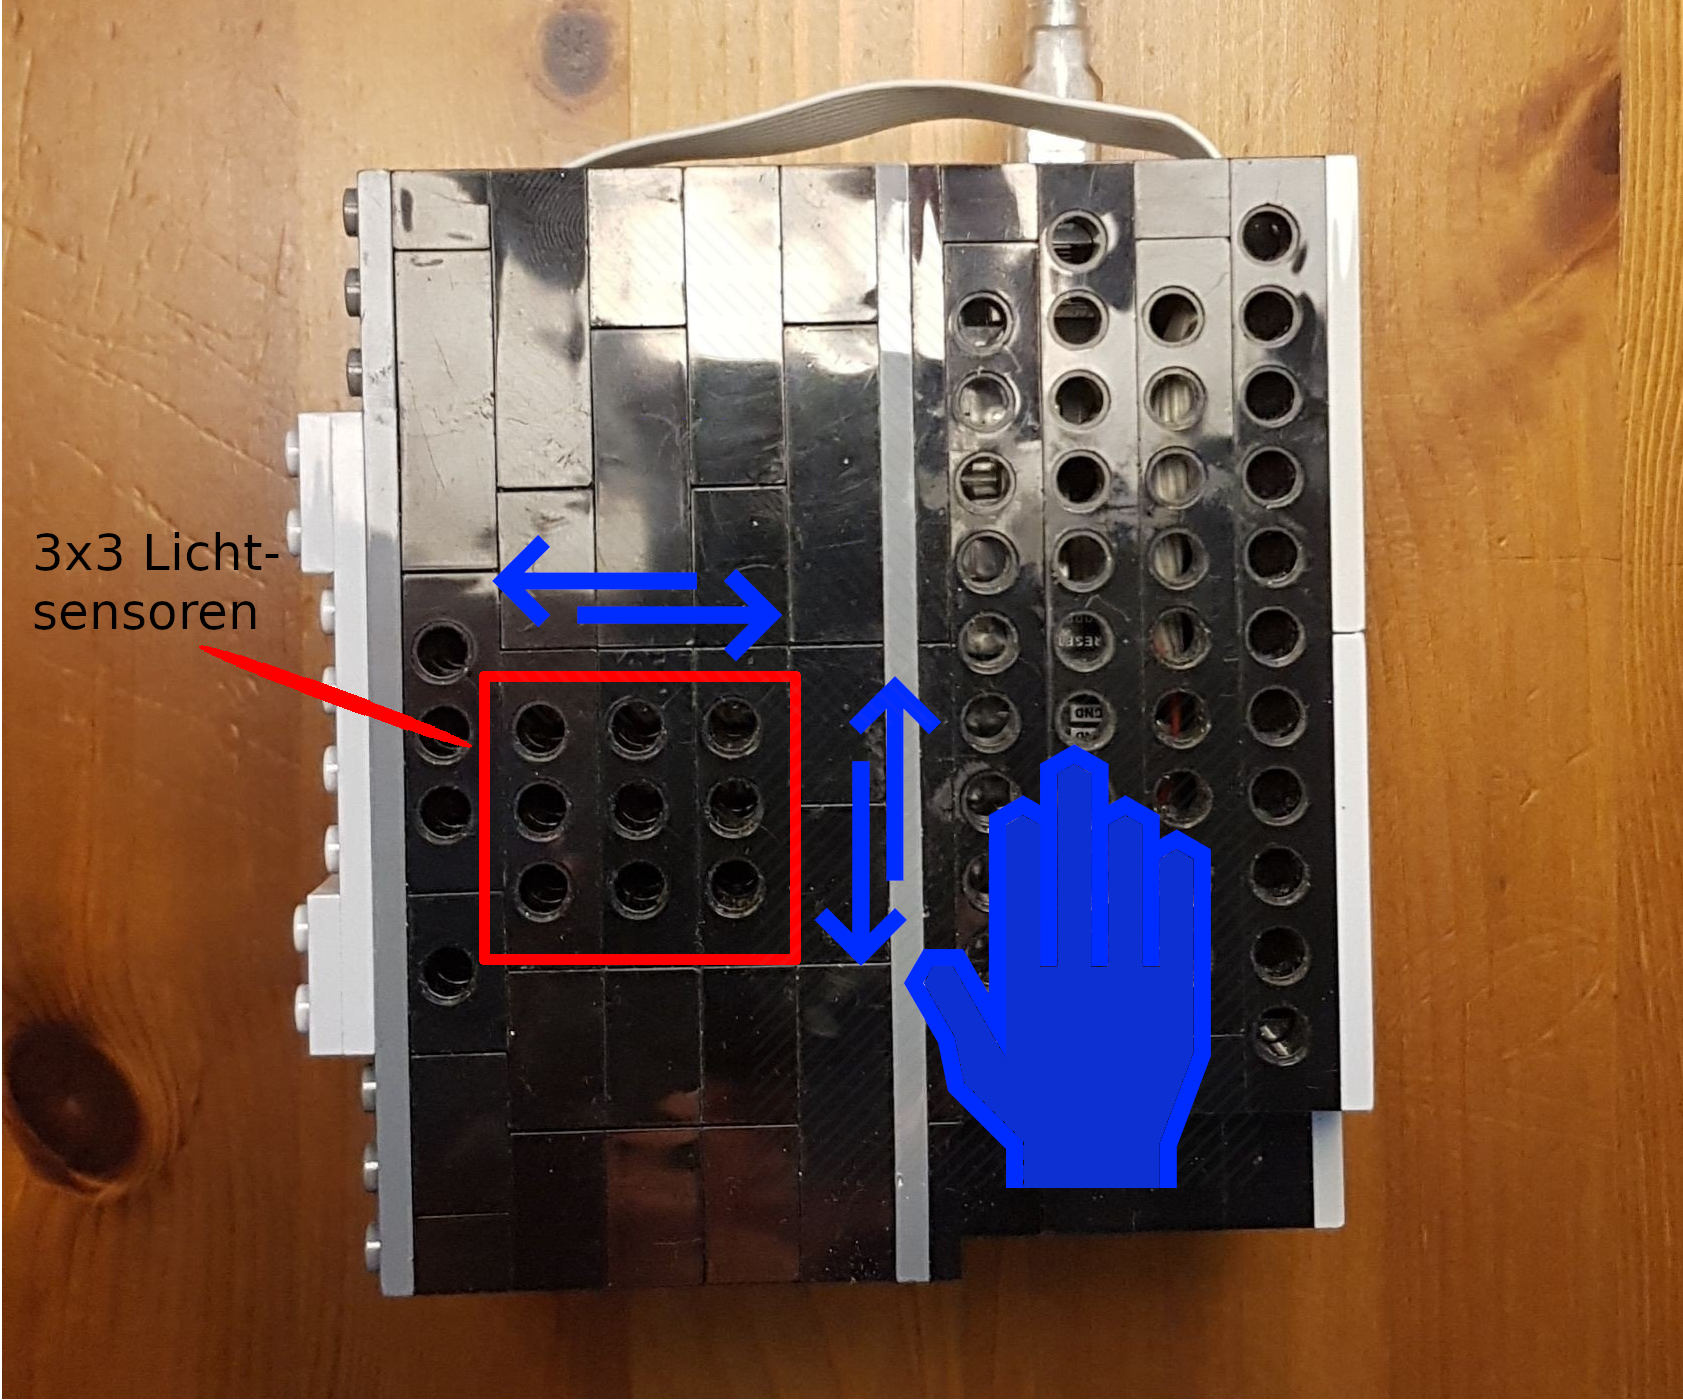
\includegraphics[width=0.9\linewidth]{aufgabe.png}
  \end{figure}
\end{frame}

\section{Entscheidungsbäume}
\begin{frame}{Entscheidungsbäume}
\begin{figure}
    \centering
    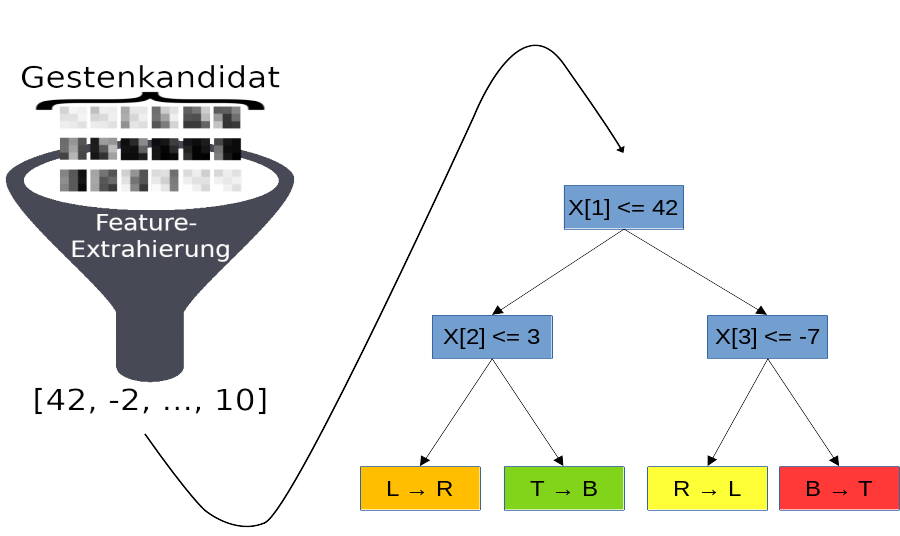
\includegraphics[width=\linewidth]{process_draw.png}
\end{figure}
\end{frame}

\section{Hauptteil}
\begin{frame}{Was wurde gemacht?}
\begin{itemize}
    \item 30 verschiedene Features
    \item 5 verschiedene Ensemble-Methoden
    \item Insgesamt 22528 Konfigurationen evaluiert
    \item Trainingsdaten von Kubik und Feng erweitert
    \item Verglichen mit Testdaten von Klisch
    \item Programmgröße, Klassifizierungsgenauigkeit und Ausführungsgeschwindigkeit evaluiert
    \item Beste Feature-Menge: Schwerpunktverteilung
\end{itemize}
\end{frame}

\begin{frame}{Schwerpunktverteilung - Schwerpunkt}
\begin{figure}
    \begin{minipage}[c]{0.5\linewidth}
        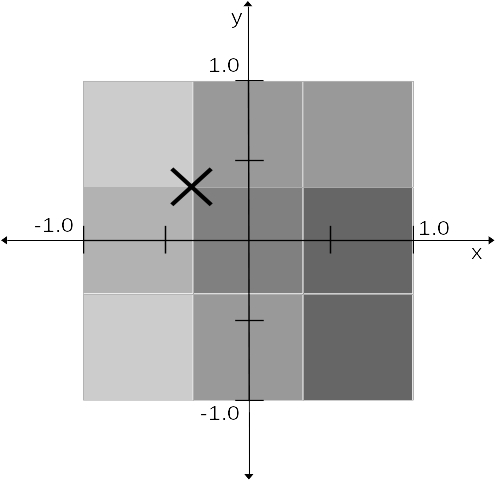
\includegraphics[width=\linewidth]{schwerpunkt_ansatz.jpg}
    \end{minipage}
    \hfill
    \begin{minipage}[c]{0.3\linewidth}
        $\begin{pmatrix}
            p_{00} & p_{01} & p_{02}\\
            p_{10} & p_{11} & p_{12}\\
            p_{20} & p_{21} & p_{22}
        \end{pmatrix}$
        \\\\\\
        $P = \sum_{i,j} p_{i,j}$
        \\\\
        $X_s = \frac{\sum_{i=0}^{2} p_{i,2} - \sum_{i=0}^{2} p_{i,0}}{P}$
        \\\\
        $Y_s = \frac{\sum_{i=0}^{2} p_{0,i} - \sum_{i=0}^{2} p_{2,i}}{P}$
    \end{minipage}
\end{figure}
\end{frame}

% Nachteil: Repräsentiert nicht genau den Schwerpunkt (Approximation)
% Vorteil: Schnell und Speichereffizient, da partiell verarbeitbar
\begin{frame}{Schwerpunktverteilung}
    \centering
    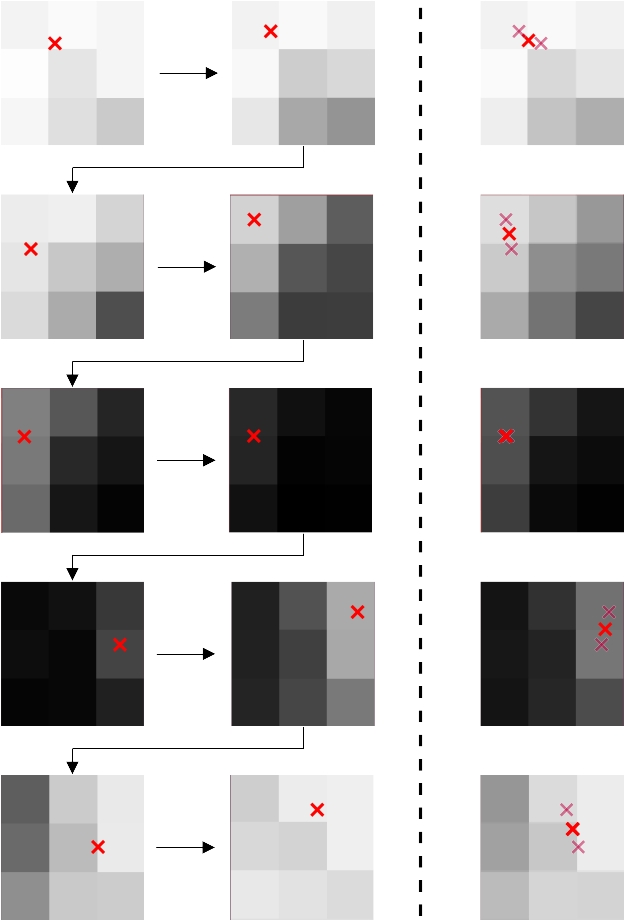
\includegraphics[width=0.5\linewidth]{schwerpunktverteilung.jpg}
\end{frame}

\begin{frame}{Schwerpunktverteilung mit Gleitkommazahlen}
    \hspace*{-0.5cm}
    \begin{tabular}{ | p{4cm} | c | c | c | c |}
        \hline
        Konfiguration & Beste & Unter 44 kB & Unter 28 kB \\\hline
        Ensemble-Methode & Boosting & Random Forest & Random Forest  \\\hline
        Maximalhöhe & 20 & 12 & 10 \\\hline
        Waldgröße & 10 & 7 & 4 \\\hline
        Blattgröße & 8 & 1 & 2 \\\hline
        Programmgröße in Byte & 83304 & 43668 & 20188 \\\hline
        Testmenge von Klisch & 94,8\% & 89,6\% & 89,6\% \\\hline
        Gestentestmenge & 97,0\% & 96,5\% & 95,6\% \\\hline
        Nullgestentestmenge & 92,2\% & 92,4\% & 88,8\% \\\hline
    \end{tabular}
\end{frame}

\begin{frame}{Schwerpunktverteilung mit Ganzzahlen}
    \centering
    \begin{tabular}{ | l | c | c | c |}
        \hline
        Konfiguration & Beste & Unter 44 kB \& 28 kB \\\hline
        Ensemble-Methode & ExtraTrees & Random Forest \\\hline
        Maximalhöhe & 21 & 13 \\\hline
        Waldgröße & 11 & 7 \\\hline
        Blattgröße & 2 & 4 \\\hline
        Programmgröße in Byte & 76200 & 21532 \\\hline
        Testmenge von Klisch & 95,8\% & 91,7\% \\\hline
        Gestentestmenge & 98,8\% & 97,1\% \\\hline
        Nullgestentestmenge & 95,6\% & 94,5\% \\\hline
    \end{tabular}
\end{frame}

\begin{frame}{Kombinierte Schwerpunktverteilung}
    \centering
    \begin{tabular}{ | p{4cm} | c | c | c | c |}
        \hline
        Konfiguration & Beste & Unter 44 kB & Unter 28 kB \\\hline
        Schwerpunktverteilung Gleitkommazahl & Beste & Unter 14 kB & Unter 14 kB \\\hline
        Schwerpunktverteilung Ganzzahlen & Beste &  Unter 28 kB & Unter 14 kB \\\hline
        Programmgröße in Byte & - & 33276 & 20252 \\\hline
        Testmenge von Klisch & 94,8\% & 87,5\% & 87,5\% \\\hline
        Gestentestmenge & 99,0\% & 97,7\% & 96,9\% \\\hline
        Nullgestentestmenge & 95,8\% & 92,9\% & 92,5\% \\\hline
    \end{tabular}
\end{frame}

\begin{frame}{Testmenge mit Offset}
    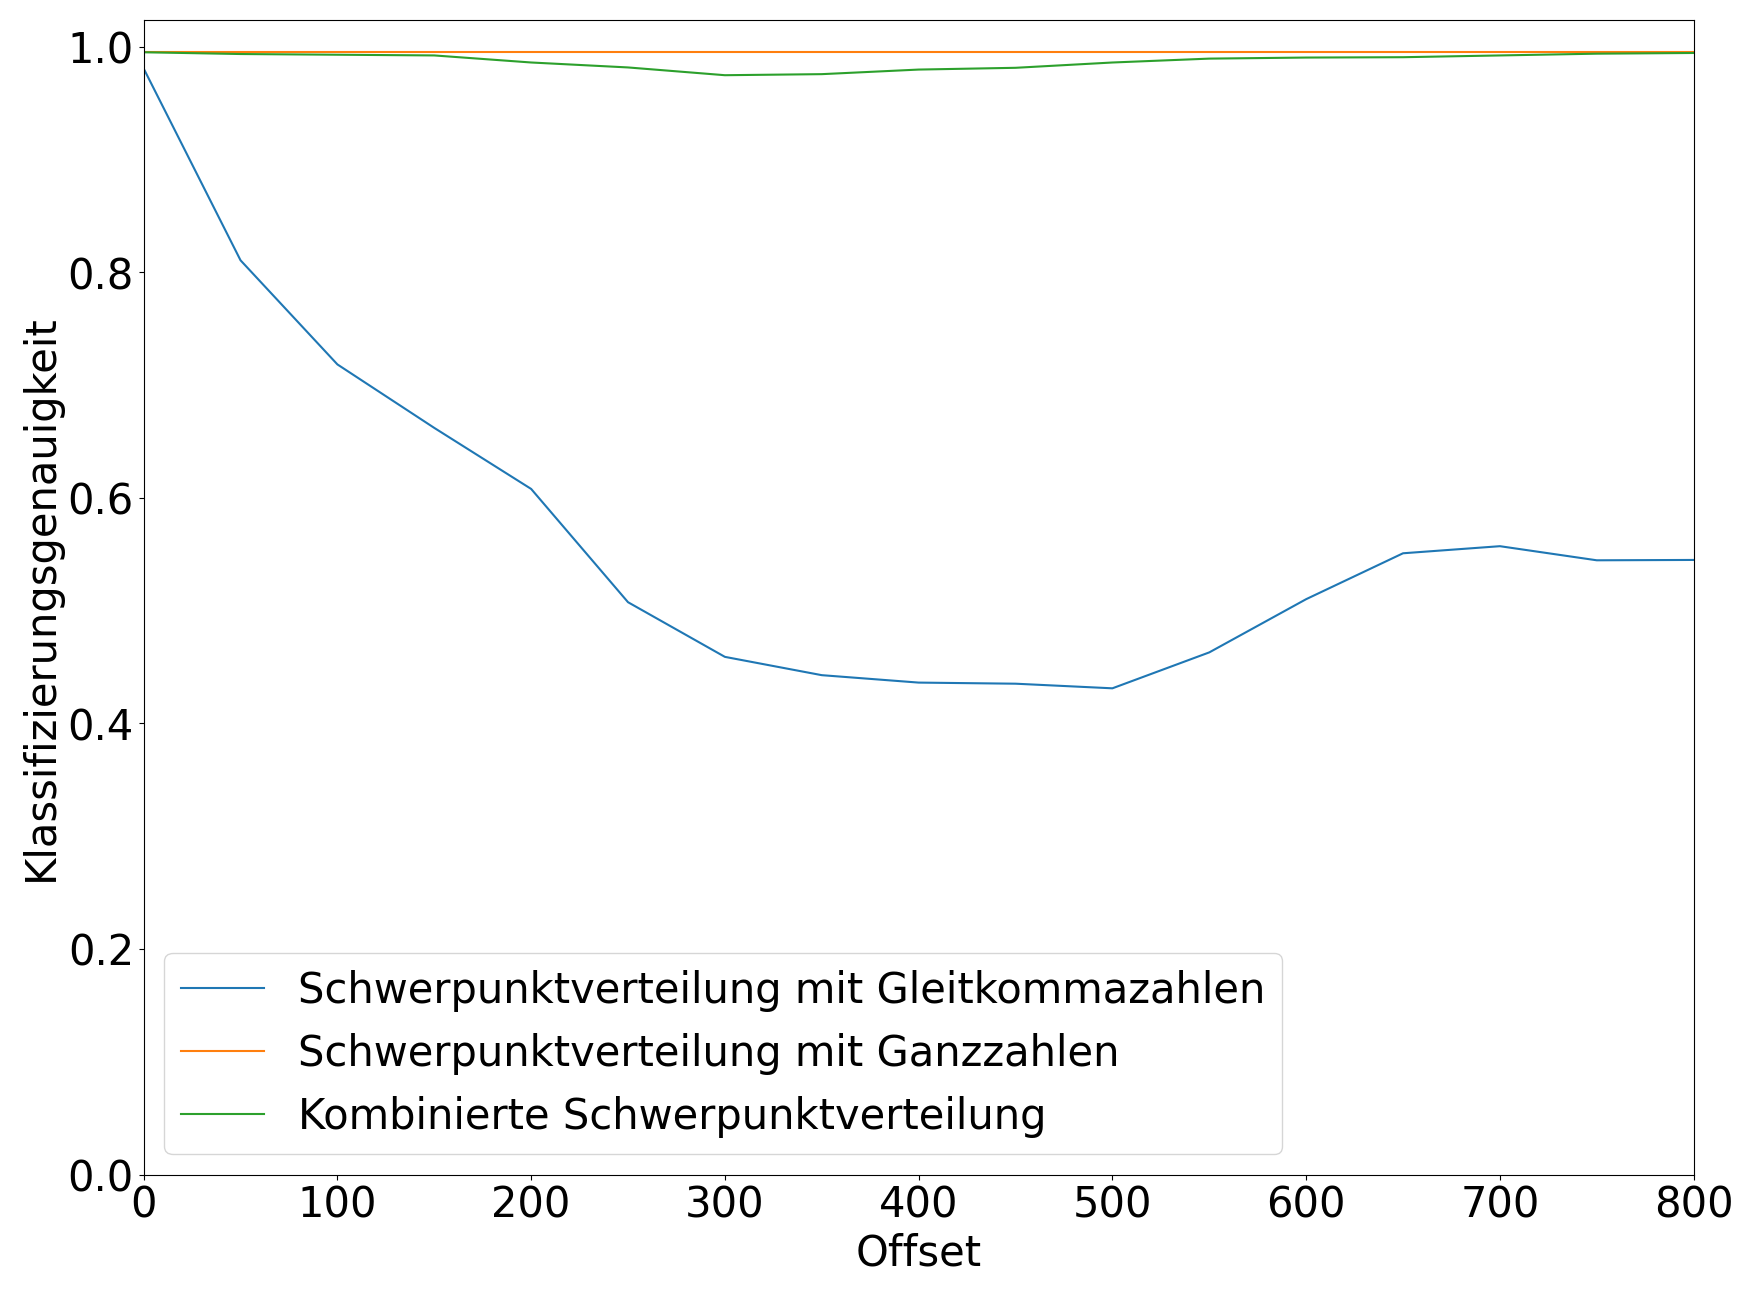
\includegraphics[width=\linewidth]{brightness_offset.png}
\end{frame}

\begin{frame}{Testmenge mit Skalierung}
    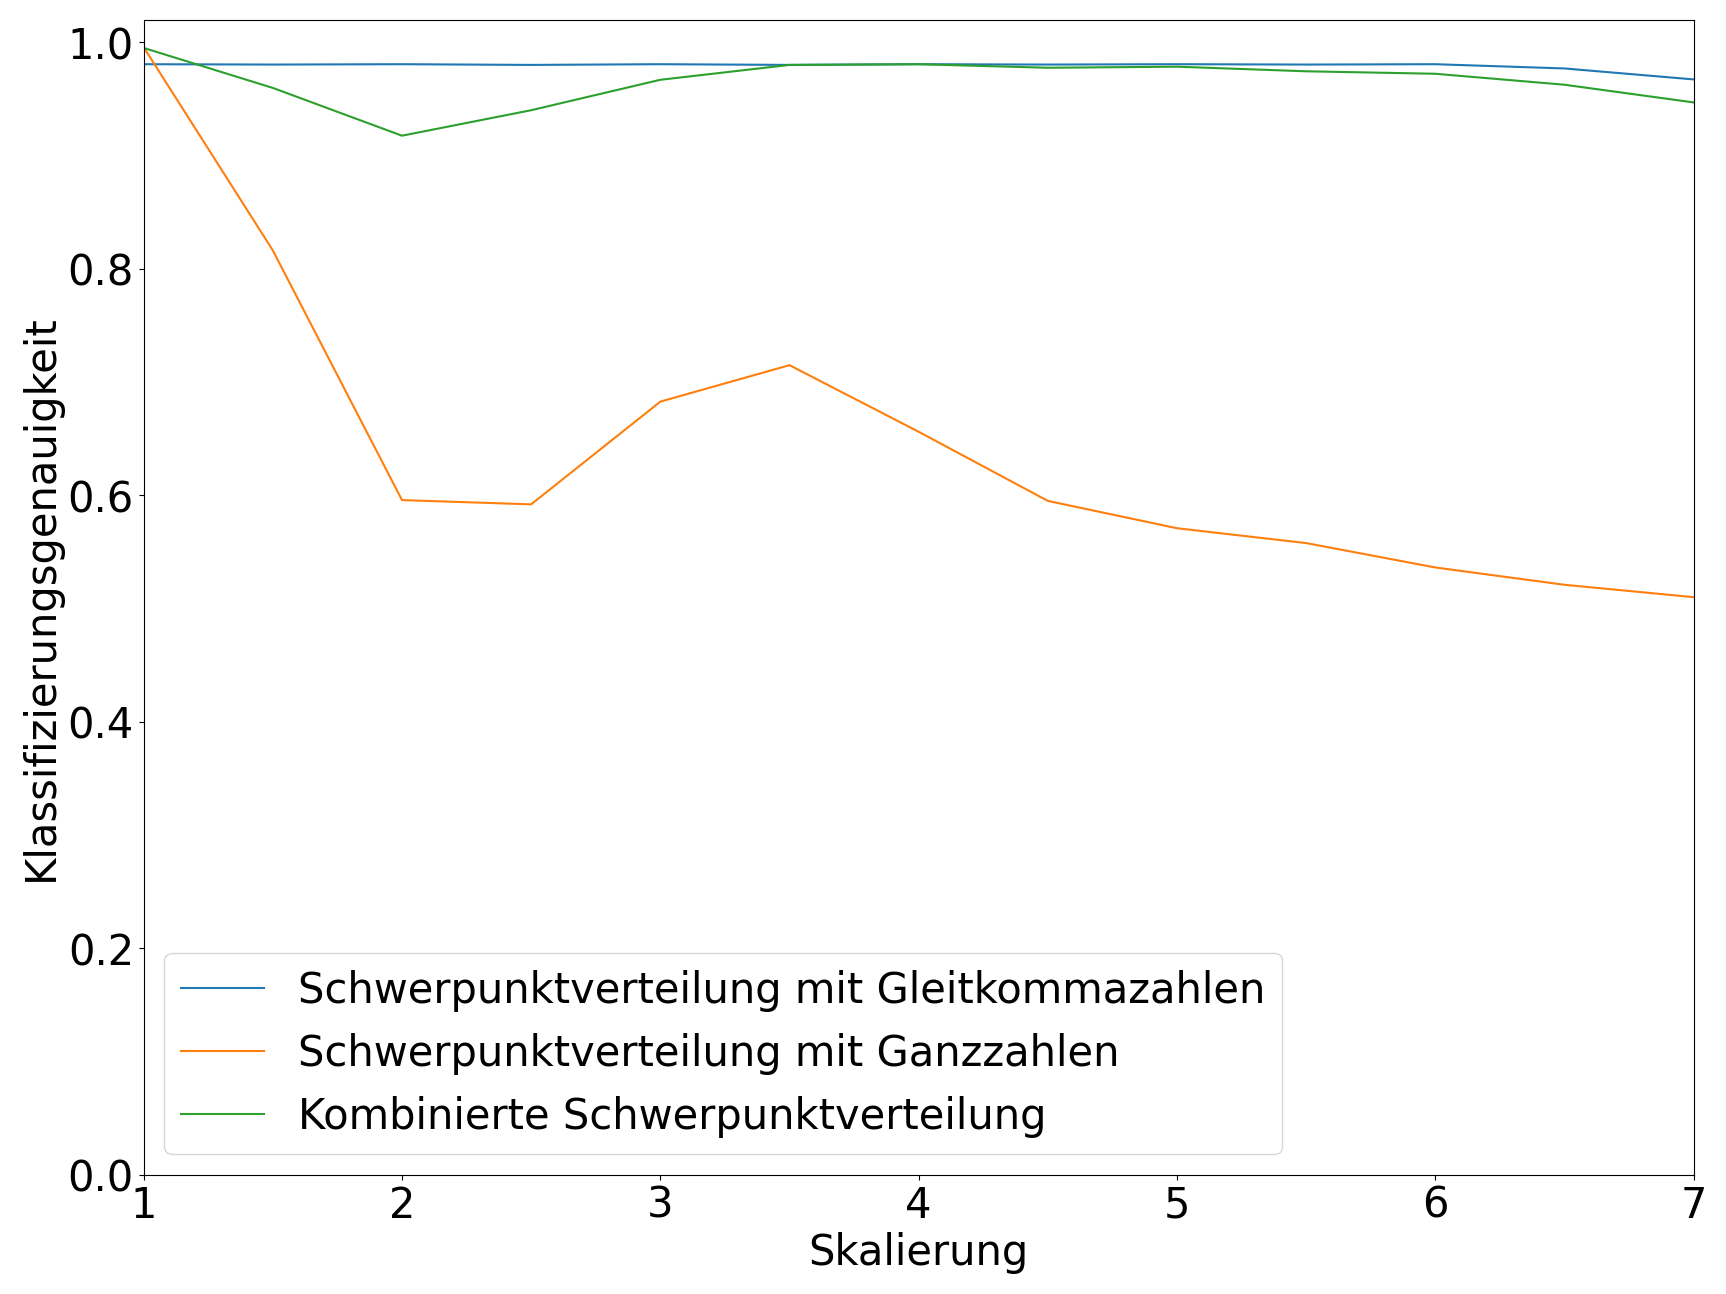
\includegraphics[width=\linewidth]{brightness_scaling.png}
\end{frame}

\begin{frame}{Testmenge mit Skalierung und konstantem Kontrast}
    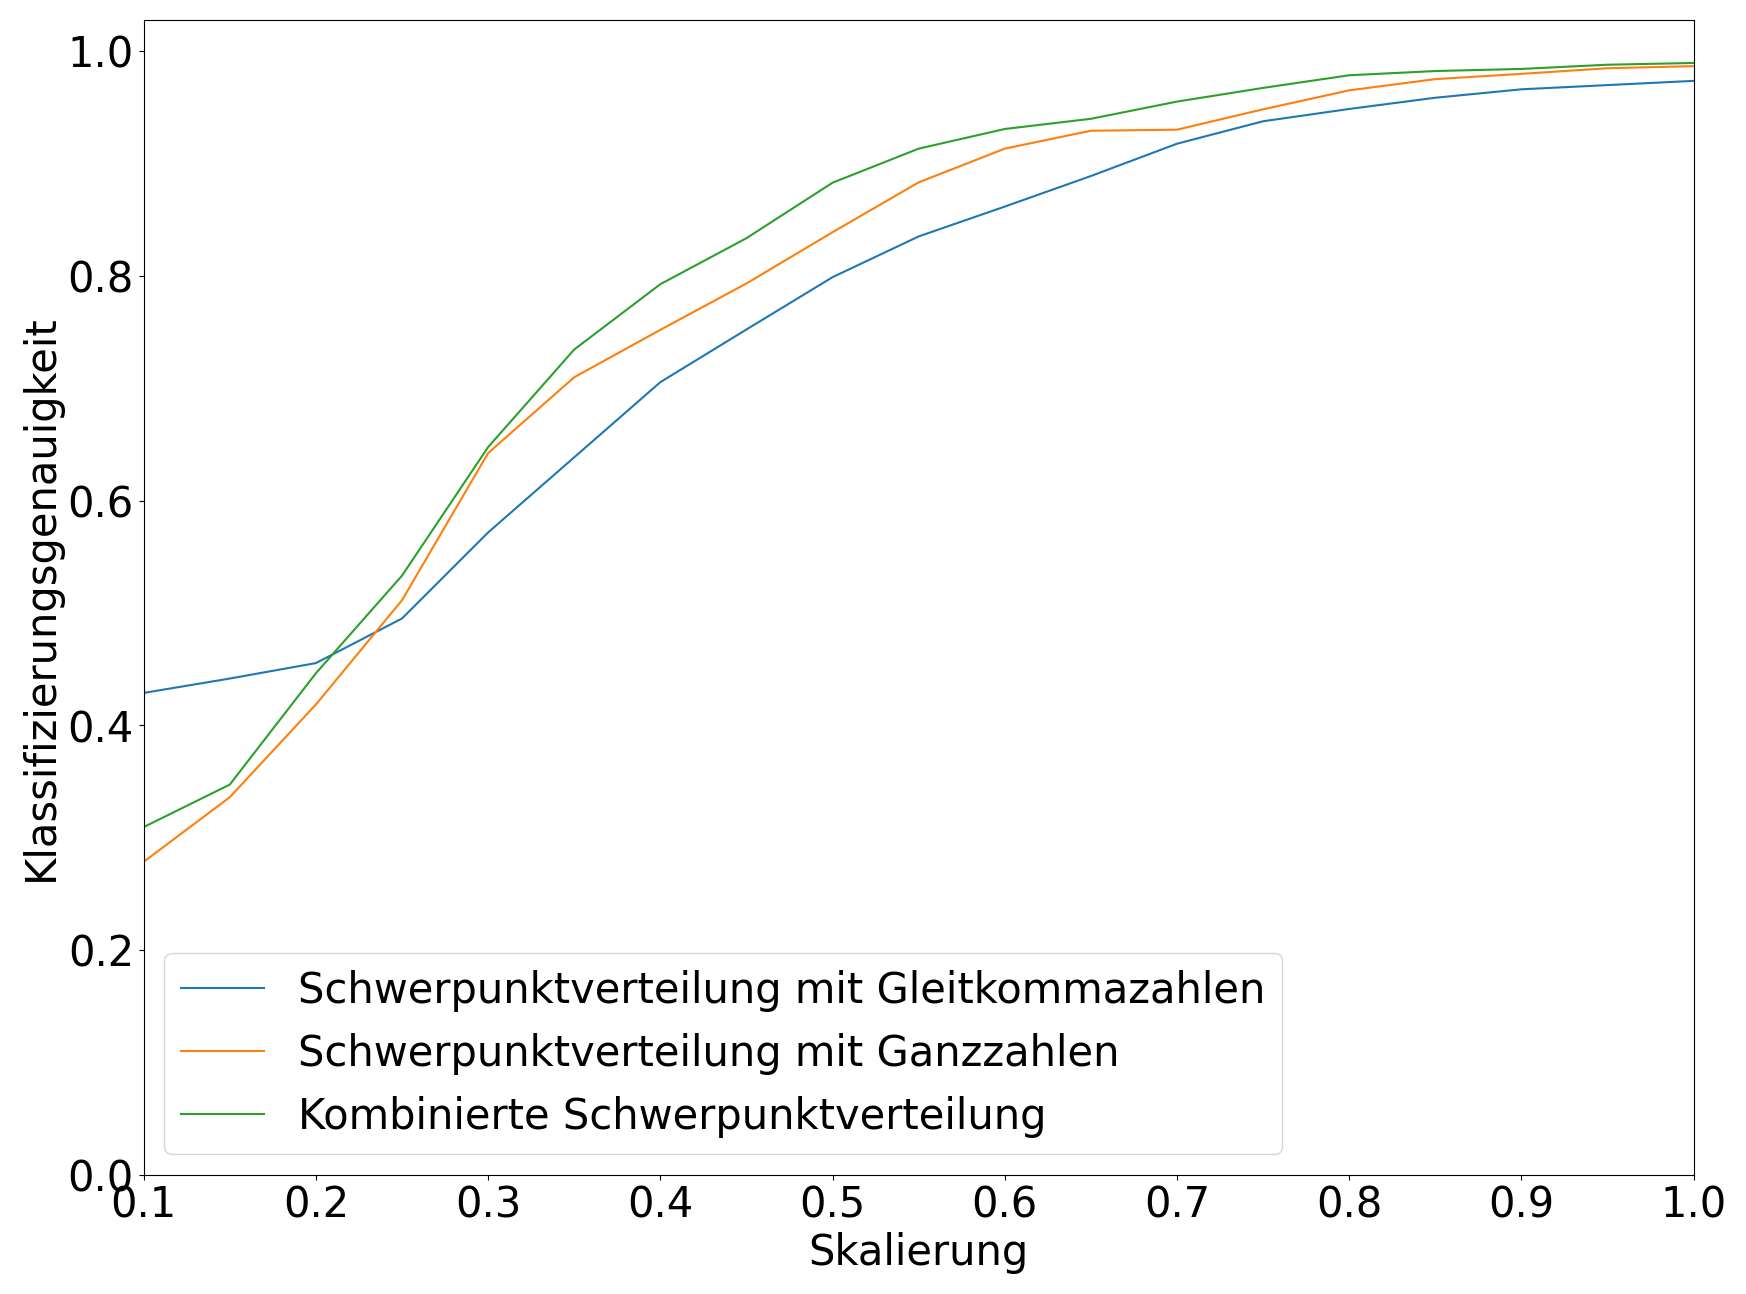
\includegraphics[width=\linewidth]{brightness2_scaling.png}
\end{frame}

% Minimierung der Zyklen pro Instruktionen und Instruktionen
% Beispiel: 100 Puffer, 10 Bäume, 20 Max Tiefe
\begin{frame}{Ausführungsgeschwindigkeit}
\begin{center}
Ausführungsgeschwindigkeit $\leq$ Feature-Extrahierung $+$ \#Bäume(Maximale-Baumhöhe $\cdot$ Vergleich) $+$ Wahlklassifizierer
\end{center}
\vspace*{0.5cm}
\centering
\begin{tabular}{|l|c|c|}
    \hline
    Operation & 16-Bit Integer & 32-Bit Float \\\hline
    Feature-Extrahierung Konstant & $173,2~\mu s$ & $273,2~\mu s$ \\\hline
    Feature-Extrahierung pro Bild & $1,1~\mu s$ & $13,7~\mu s$ \\\hline
    Wahlklassifizierer & $4~\mu s$ & $4~\mu s$ \\\hline
    Overhead pro Baum & $1,1~\mu s$ & $1,1~\mu s$ \\\hline
    Vergleich & $0,9~\mu s$ & $5,2~\mu s$ \\\hline
    WCET von Beispiel & $478,2~\mu s$ & $2698,2~\mu s$ \\\hline
\end{tabular}
\end{frame}

\begin{frame}{Schlussfolgerungen}
\begin{itemize}
    \item Hohe Klassifizierungsgenauigkeit auf Testmenge von Klisch
    \item Kann Nullgesten von validen Gesten unterscheiden
    \item Robust gegenüber schlechten Lichtverhältnissen
    \item Zwischen 3,6\% und 29,9\% der Ausführungsgeschwindigkeit des schnellsten bisherigen Ansatzes
    \item Geringe Nutzung von RAM => Größerer Bildpuffer
    \item Entscheidungsbaum- und Entscheidungswaldgröße vernachlässigbar für Ausführungsgeschwindigkeit
    \item Klassifizierungsgenauigkeit abhängig von Größe des Programmspeichers 
    \item Programmgröße stark abhängig von Datentyp und Art des Wahlklassifizierers
\end{itemize}
\end{frame}

% Wenn noch zeit ist, dann DEMO
\begin{frame}[standout]
  DEMO
\end{frame}

\begin{frame}[standout]
  Fragen?
\end{frame}

\begin{frame}{Ausführungsgeschwindigkeit Float-Operationen}
\centering
\begin{tabular}{ | c | p{4cm} | c | c |}
    \hline
    Operation & Funktion & WCET & WCET in Zyklen \\\hline
    \_\_lesf2 & Kleiner oder gleich Vergleich & 4 $\mu s$ & 64 \\\hline
    \_\_floatsisf & Konvertierung von 32-Bit Integer nach Float & 4 $\mu s$ & 64 \\\hline
    \_\_divsf3 & Division & 36 $\mu s$ & 576 \\\hline
    \_\_addsf3 & Addition & 12 $\mu s$ & 192 \\\hline
\end{tabular}
\end{frame}

\end{document}
